\documentclass[UTF8, a4paper, 11pt]{ctexart}
\usepackage{amsmath, amssymb, amsfonts}
\usepackage{geometry}
\geometry{left=2.5cm, right=2.5cm, top=3cm, bottom=3cm}
\usepackage{graphicx}
\usepackage{pifont}
\begin{document}

\begin{center}
    \textbf{绝密$\star$启用前}\\
    \vspace{0.5em}
    \Large \textbf{2026年普通高等学校招生全国统一考试}\\
    \vspace{0.5em}
    \Huge \textbf{数学}
\end{center}

\vspace{1em}

\noindent \textbf{注意事项:}\\
1. 答卷前,考生务必将自己的姓名、准考证号填写在答题卡上。\\
2. 回答选择题时,选出每小题答案后,用铅笔把答题卡上对应题目的答案标号涂黑。 如需改动,用橡皮擦干净后,再选涂其他答案标号。回答非选择题时,将答案写在答题卡上,写在本试卷上无效。\\
3. 考试结束后,将本试卷和答题卡一并交回。

\vspace{1em}
\hrule
\vspace{1em}

\section*{一、选择题:本题共8小题,每小题5分,共40分。在每小题给出的四个选项中,只有一项是符合题目要求的。}

\noindent 1. 样本数据 $6,8,4,5,12$ 的中位数为
\begin{itemize}
    \item A. 5
    \item B. 6
    \item C. 8
    \item D. 9
\end{itemize}

\noindent 2. 已知平面向量 $a,b$ 不共线,且 $2a+yb=xa-3b$ 则
\begin{itemize}
    \item A. $x=2,y=-3$
    \item B. $x=-2,y=3$
    \item C. $x=2,y=3$
    \item D. $x=-2,y=-3$
\end{itemize}

\noindent 3. 已知集合 $A=\{\sin(\frac{7\pi}{6}),\cos(\frac{5\pi}{3}),\tan(\frac{5\pi}{4})\}$, $B=\{-\frac{\sqrt{3}}{2},-\frac{1}{2},1\}$,则 $A\cap B=$
\begin{itemize}
    \item A. $\{-\frac{\sqrt{3}}{2},-\frac{1}{2}\}$
    \item B. $\{-\frac{\sqrt{3}}{2},1\}$
    \item C. $\{-\frac{1}{2},1\}$
    \item D. $\{-\frac{\sqrt{3}}{2},-\frac{1}{2},1\}$
\end{itemize}

\noindent 4. 曲线 $y=5x+8\ln x$ 在点 $(1,5)$ 处的切线方程为
\begin{itemize}
    \item A. $y=3x+2$
    \item B. $y=5x$
    \item C. $y=8x-3$
    \item D. $y=13x-8$
\end{itemize}

\noindent 5. 已知抛物线 $C_{1}:y^{2}=2p_{1}x(p_{1}>0)$ 和 $C_{2}:x^{2}=2p_{2}y(p_{2}>0)$ 均经过点 $(4,8)$,则 $C_{1}$ 的焦点与 $C_{2}$ 的焦点之间的距离为
\begin{itemize}
    \item A. 12
    \item B. $4\sqrt{5}$
    \item C. 6
    \item D. $\frac{\sqrt{65}}{2}$
\end{itemize}

\noindent 6. 已知函数 $f(x)=\frac{x+2}{e^{x}+a}$ 最大值为1,则 $a=$
\begin{itemize}
    \item A. $\frac{1}{2}$
    \item B. 1
    \item C. $\frac{3}{2}$
    \item D. 2
\end{itemize}

\noindent 7. 一百零八塔位于宁夏回族自治区青铜峡市,以其独特的建筑格局和深远的历史文化闻名遐迩,该塔群共有108座塔,依山势自上而下排成12行,将第 $i$ 行中塔的座数记为 $a_{i}(i=1,2,\dots,12)$,其中 $a_{1}=1,a_{2}=a_{3}=3,a_{4}=a_{5}=5$,且 $a_{6},a_{7},\dots,a_{12}$ 是一个首项为7,公差为2的等差数列,将 $a_{1},a_{2},\dots,a_{12}$ 分为6组,每组2个数,使得每组的2个数之和可构成一个项数为6且公差为 $d(d>0)$ 的等差数列,则 $d=$
\begin{itemize}
    \item A. 2
    \item B. 4
    \item C. 6
    \item D. 8
\end{itemize}

\noindent 8. 设 $U=\{(x_{1},x_{2},x_{3}) \mid x_{i}\in\{-2,-1,1,2\},i=1,2,3\}$ 为空间中64个点构成的集合,记 $P(1,1,1)$,记样本空间 $\Omega=\complement_{U}\{P\}$,从中随机取一个点,定义随机变量 $X$ 如下:对 $\Omega$ 中的每个点 $A(x_{1},x_{2},x_{3})$,令 $X(A)=x_{1}+x_{2}+x_{3}.$ 则 $X$ 的数学期望为
\begin{itemize}
    \item A. $-\frac{1}{21}$
    \item B. $-\frac{1}{63}$
    \item C. 0
    \item D. $\frac{1}{7}$
\end{itemize}

\vspace{1em}

\section*{二、选择题:本题共3小题,每小题6分,共18分。在每小题给出的选项中,有多项符合题目要求。全部选对的得6分,部分选对的得部分分,有选错的得0分。}

\noindent 9. 设 $z=3+2i,$ 则
\begin{itemize}
    \item A. $\overline{z}=3-2i$
    \item B. $|z|=5$
    \item C. $z^{2}=5+12i$
    \item D. $\frac{z+3}{z-i}\in\mathbb{R}$
\end{itemize}

\noindent 10. 在空间中, $A,B$ 为两个定点,动点 $C$ 到直线 $AB$ 的距离为2,动点 $D$ 到直线 $AB$ 的距离为1,若二面角 $C-AB-D$ 为 $60^{\circ}$,则
\begin{itemize}
    \item A. $\angle CAD\ge60^{\circ}$
    \item B. $CD\ge\sqrt{3}$
    \item C. 当 $AB\perp CD$ 时, $CD\perp$ 平面 $ABD$
    \item D. 当 $AB\perp$ 平面 $ACD$ 时, $AC\perp AD$
\end{itemize}

\noindent 11. 已知圆 $C_{1}:(x+1)^{2}+y^{2}=1$,圆 $C_{2}:(x-1)^{2}+y^{2}=1$,圆 $C_{3}:x^{2}+(y-\sqrt{3})^{2}=1$,直线 $l:y=kx+b$ 与 $C_{1},C_{2},C_{3}$ 均有两个交点,记 $l$ 被 $C_{1},C_{2},C_{3}$ 截得的弦长分别为 $s_{1},s_{2},s_{3}.$ 则
\begin{itemize}
    \item A. $k$ 可以取任意实数
    \item B. 满足 $s_{1}=s_{2}=s_{3}$ 的直线 $l$ 共有3条
    \item C. 满足 $s_{1}+s_{2}+s_{3}=1$ 的直线 $l$ 多于3条
    \item D. 当 $b=0$ 时, $s_{1}+s_{2}+s_{3}$ 的最大值为 $\frac{2\sqrt{21}}{3}$
\end{itemize}

\vspace{1em}

\section*{三、填空题:本题共3小题,每小题5分,共15分。}

\noindent 12. 双曲线 $5x^{2}-6y^{2}=1$ 的离心率为 \underline{\hspace{2cm}}

\vspace{0.5em}
\noindent 13. 已知 $f(x)=2\sin(ax+\theta)(a\in\mathbb{Z},0\le\theta<2\pi)$ 是偶函数, $f(x)$ 在区间 $(0,\frac{\pi}{2})$ 单调递增,则 $\theta=$ \underline{\hspace{2cm}}, $f(\frac{2\pi}{3})=$ \underline{\hspace{2cm}}.

\vspace{0.5em}
\noindent 14. 设实数 $q$ 满足:存在数列 $\{a_{n}\}$,使得对于任意 $n\in\mathbb{N}^{*}$,均有 $a_{1}+a_{2}+\dots+a_{3n}=n^{2}+n,$ 且 $\{a_{n}\}$ 中有某连续9项 $a_{i},a_{i+1},\dots,a_{i+8}$ 是公比为 $q$ 的等比数列,则 $q$ 的最大值为 \underline{\hspace{2cm}}

\vspace{1em}

\section*{四、解答题:本题共5小题,共77分。解答应写出文字说明、证明过程或演算步骤。}

\noindent \textbf{15.(13分)}\\
如图,在直三棱柱 $ABC-A_{1}B_{1}C_{1}$ 中, $\angle ACB=90^{\circ}$, $AC=BC,D,E$ 分别为 $AB,A_{1}C_{1}$ 的中点.\\
\begin{center}
    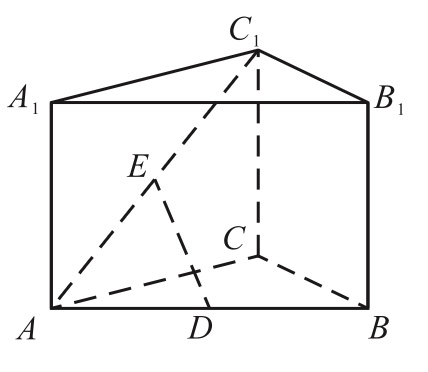
\includegraphics[width=0.4\textwidth]{1.jpg}
\end{center}
(1) 证明: $DE\parallel$ 平面 $BCC_{1}B_{1}$;\\
(2) 设 $CC_{1}=2$,直线 $DE$ 与平面 $ACC_{1}A_{1}$ 所成的角为 $45^{\circ}$,求直线 $DE$ 到平面 $BCC_{1}B_{1}$ 的距离.

\vspace{1em}
\noindent \textbf{16.(15分)}\\
已知在 $\triangle ABC$ 中, $AB=3$, $BC=2\sqrt{3}$, $\cos B=\frac{\sqrt{3}}{3}$\\
(1) 求 $\cos A$;\\
(2) 设 $D,E$ 两点满足: $D$ 在 $BA$ 的延长线上, $DE\parallel BC$, $AE\perp AC$. 若 $DE=\sqrt{6}$,求 $CE$.

\vspace{1em}
\noindent \textbf{17. (15分)}\\
设整数 $N\ge2$. 某同学用一个球进行投篮练习,至多投置 $N$ 次,当且仅当投中1次时或 $N$ 次均未投中时,停止练习,设该同学每次投中的概率为 $p(0<p<1)$,各次投中与否相互独立.记 $X$ 为停止练习时该同学的投篮次数.\\
(1) 当 $N=4,p=\frac{1}{3}$ 时,求 $X$ 的分布列;\\
(2) 设 $k,m$ 均为自然数.\\
(i) 当 $k\le N-1$ 时,求 $P(X>k)$;\\
(ii) 当 $k+m\le N-1$ 时,证明: $P(X>k+m \mid X>k)=P(X>m).$

\vspace{1em}
\noindent \textbf{18.(17分)}\\
已知椭圆 $C:\frac{x^{2}}{a^{2}}+\frac{y^{2}}{b^{2}}=1(a>b>0)$ 的左焦点为 $F(-1,0)$,离心率为 $\frac{1}{2}.$\\
(1) 求 $C$ 的方程;\\
(2) 设 $O$ 为坐标原点,过 $F$ 且斜率大于 $0$ 的动直线 $l$ 与 $C$ 交于 $P,Q$ 两点,其中 $Q$ 在第三象限,直线 $PO$ 与 $C$ 的另一个交点为 $R$.\\
(i) 若 $\triangle PQR$ 的面积是 $\triangle PFO$ 的面积的3倍,求 $l$ 的方程;\\
(ii) 求 $\tan\angle PQR$ 的最小值.

\vspace{1em}
\noindent \textbf{19.(17分)}\\
已知函数 $f(x)$ 的定义域为 $\mathbb{R}$,且当 $x<0$ 时 $f(x)=2^{x}$. 对任意 $x_{0}\in\mathbb{R}$,定义集合 $D(x_0)=\{d\in\mathbb{R} \mid f(x_0+d)>f(x_0)\}.$\\
(1) 若当 $x\ge0$ 时, $f(x)=1-x$,求 $D(-1)$;\\
(2) 若 $f(x)$ 是奇函数, $f(x_{1})\le f(x_{2})$,且 $x_{1}x_{2}\ne0$,证明: $D(x_{2})\subseteq D(x_{1})$;\\
(3) 设 $f(x)$ 满足:\ding{172}若 $f(x_{1})\le f(x_{2})$,则 $D(x_{2})\subseteq D(x_{1})$;\ding{173}当 $0<x<1$ 时, $f(x)<f(0)$.\\
(i) 证明: $f(0)\ge1$;\\
(ii) 证明: $f(x)$ 在区间 $(0,+\infty)$ 单调递增.

\end{document}